\chapter{Regression} \label{ch:regression}

Regression is one of the most fundamental and important applications of AI. This chapter introduces regression and corresponding artificial neural networks structures.

\section{Linear Regression} \label{sec:linear_regression}

Linear regression is one of the most basic problems of AI. Though simple, it plays a significant part in the history of AI. The methodologies used in linear regression, such as gradient descent, inspire the further development of more sophisticated artificial neural networks structures.

\subsection{Problem Statement}

Let
\begin{eqnarray}
	y &=& f(x, \epsilon) \label{eq:linear_regression_problem}
\end{eqnarray}
where $y\in\mathbb{R}$ the output, $x\in\mathbb{R}^n$ the inputs in vector form (also known as the features), $n$ the number of features, $\epsilon$ the stochasticity of the model, and $f(\cdot)$ an unknown function of $x$. The purpose of linear regression is to find such $\theta \in \mathbb{R}^n$ and $\theta_0\in\mathbb{R}$ for
\begin{eqnarray}
	h(x) &=& \theta^T x + \theta_0 \label{eq:linear_regression}
\end{eqnarray}
such that $h(x)$ is an approximation of $y$ with minimum $\norm{y-h(x)}$.

\begin{mdframed}
\noindent \textbf{Linear Regression Equation with Augmented State}

Technically speaking, \eqref{eq:linear_regression} is not a linear function of $x$ due to the bias term $\theta_0$. One can make it a linear function using augmented state vector as follows.

Let
\begin{eqnarray}
	\bar{x} &=& \left[\begin{array}{cc}
		x_0 & x^T
	\end{array}\right]^T \nonumber \\
	\bar{\theta} &=& \left[\begin{array}{cc}
		\theta_0 & \theta^T
	\end{array}\right]^T \nonumber
\end{eqnarray}
with $x_0=1$ a constant augmented parameter. Equation \eqref{eq:linear_regression} then becomes
\begin{eqnarray}
	h(x) &=& \bar{\theta}^T\bar{x} \label{eq:linear_regression_linear}
\end{eqnarray}
which is a linear function of $\bar{x}$.

If often does not batter which notation to use, either \eqref{eq:linear_regression} or \eqref{eq:linear_regression_linear}, so long as it is used consistently.

\end{mdframed}

\subsection{Solution with Gradient Descent}

As a first step, collect training samples. Let there be $m$ training samples denoted by $(x^{(i)}, y^{(i)})$, $i=1,\ldots,m$.

With the $m$ samples, $\theta$ and $\theta_0$ can be determined as follows.
\begin{eqnarray}
	\theta, \theta_0 &=& \argmin_{\theta, \theta_0} J \label{eq:linear_regression_solution} \\
	J &=& \dfrac{1}{2} \sum_{i=1}^{m} \left(h\left(x^{(i)}\right)-y^{(i)}\right)^2 \nonumber \\
	&=& \dfrac{1}{2} \sum_{i=1}^{m} \left(\theta^T x^{(i)} + \theta_0 -y^{(i)}\right)^2 \label{eq:linear_regression_solution_j}
\end{eqnarray}
with $J$ the quadratic cost function.

\begin{mdframed}
\noindent \textbf{Why quadratic error in cost function \eqref{eq:linear_regression_solution_j}?}

Using quadratic error in \eqref{eq:linear_regression_solution_j} gives us certain benefits, such as \eqref{eq:linear_regression_solution_j} becoming convex and differentiable.

Furthermore, if in \eqref{eq:linear_regression_problem}, the noise $\epsilon$ is Gaussian distribution and added to the measurement, by using quadratic error in \eqref{eq:linear_regression_solution_j}, \eqref{eq:linear_regression_solution} becomes the maximum likelihood estimation of the parameters $\theta$ and $\theta_0$. It is the optimal estimation and gives the minimum estimation error variance. 

The proof can be found on control system relevant notebooks and is neglected here.

\end{mdframed}

There are different ways to solve \eqref{eq:linear_regression_solution}. For example, since the analytical form of $J$ in \eqref{eq:linear_regression_solution_j} is known, we can solve $\frac{\partial J}{\partial \theta}=0$ and $\frac{\partial J}{\partial \theta_0}=0$ to get $\theta$ and $\theta_0$. The result is given by the \mync{normal equation} below.
\begin{eqnarray}
	X^TX\theta &=& X^TY \nonumber \\
	X_{m\times n} &=& \left[\begin{array}{ccc}
		x_1^1 & \ldots & x_n^1 \\
		\vdots & \ddots & \vdots \\
		x_1^m & \ldots & x_n^m 
	\end{array}\right] \nonumber \\
	Y_{m \times 1} &=& \left[\begin{array}{c}
		y^1 \\ \vdots \\ y^m
	\end{array}\right] \nonumber
\end{eqnarray}
solving which gives
\begin{eqnarray}
	\theta &=& \left(X^TX\right)^{-1}X^TY
\end{eqnarray}
which is known as the \mync{least squares estimation} of $\theta$.

For the scope of this chapter, consider using gradient decent as follows. Gradient decent may seem overkill for linear regression problem, but it is so widely used in machine learning and it is worth introducing here.

In \mync{gradient descent}, initialize $\theta$ and $\theta_0$ randomly or to be zero, and use them as a starting point. Iteratively do the following. Calculate the gradient of $J$ at $(\theta,\theta_0)$ and revised $\theta$ and $\theta_0$ in the inverse direction of the gradient to get a smaller value of $J$ as follows.
\begin{eqnarray}
	\theta &\leftarrow& \theta - \alpha \dfrac{\partial}{\partial \theta} J \nonumber \\
	\theta_0 &\leftarrow& \theta_0 - \alpha \dfrac{\partial}{\partial \theta_0} J \nonumber
\end{eqnarray}
where $\alpha$ is the \mync{learning rate} which is often a small value, and from \eqref{eq:linear_regression_solution_j}
\begin{eqnarray}
	 \dfrac{\partial}{\partial \theta_j} J &=& \sum_{i=1}^{m} \left[\left(h\left(x^{(i)}\right)-y^{(i)}\right)x_j^{(i)}\right] \label{eq:linear_regression_gradient}
\end{eqnarray}
with $j=0,...,n$ and $x_0=1$.

Iterate until $\theta$ and $\theta_0$ converge, or until a maximum iteration number is reached, or until $J$ does not decrease further.

Notice that in each iteration, all the training samples are used to calculate $\dfrac{\partial}{\partial \theta}J$ and $\dfrac{\partial}{\partial \theta_0}J$ in the gradient descent. This is known as \mync{batch gradient descent}. When the total number of samples $m$ is extremely large, batch gradient descent requires large computer memory. To save computational resources in the case the training set is very large, consider using \mync{mini-batch gradient descent}, where the $m$ training samples are divided into smaller mini batches. In each iteration, one of the mini-batch is used. It will take several iterations before the entire training samples are gone through. In the special case where there is only one sample in each mini-batch, the method is known as the \mync{stochastic gradient descent}.

In general, batch gradient descent consumes more computational resources in each iteration than mini-batch or stochastic gradient descent and hence it is often very slow. However, it is more robust and helps with more stable parameter converges. When using mini-batch and stochastic gradient descent, on the other hand, the parameters may never truly asymptotically converge. Instead, they may circulate in a very small zone. Nowadays for many applications the training set is often very large, making it impractical to use batch gradient descent. Mini-batch and stochastic gradient descent are more often used. Though there is the risk that they may not asymptotically converge to the minimum, the result is often acceptable.

Each time the entire training set is scanned, it is called an \mync{epoch}. In batch gradient descent, each iteration corresponds with an epoch, whereas in mini-batch gradient descent, multiple iterations correspond with an epoch.

A demonstrative example is given in Fig \ref{fig:linear_regression_exp}. In this $1$-D linear regression example, a straight line is used to fit $50$ samples as shown by the red crosses. A total number of $20$ epochs are used in the training. The result is given by the blue solid line.

\begin{figure}[!htb]
	\centering
	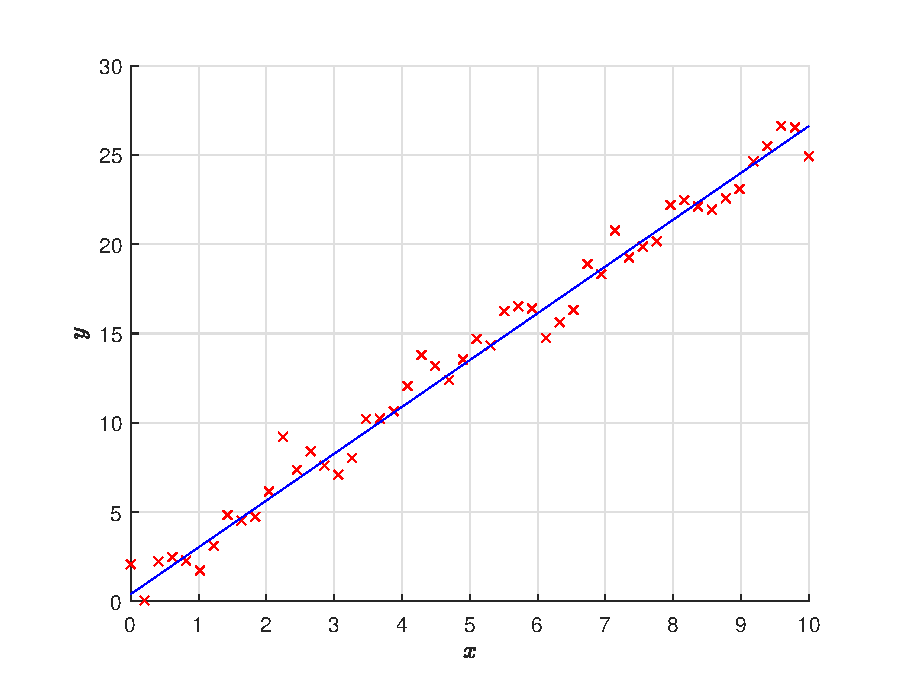
\includegraphics[width=0.6\textwidth]{chapters/part-1/figures/linear_regression_exp.eps}
	\caption{A demonstrative example for $1$-D linear regression, where a straight line is used to fit $50$ samples, with the results after $5$, $10$ and $20$ epochs of training are given by the blue dot line, dash dot line and solid lines respectively.} \label{fig:linear_regression_exp}
\end{figure}

During the training, the cost function \eqref{eq:linear_regression_solution_j} decreases as the line fits into the samples. This is reflected by Fig. \ref{fig:linear_regression_exp_j}. As a demonstration of how training improves the results, the intermediate result after $5$ epochs and $10$ epochs of training are given in Fig \ref{fig:linear_regression_exp} by the blue dot line and the blue dash dot line respectively.

\begin{figure}[!htb]
	\centering
	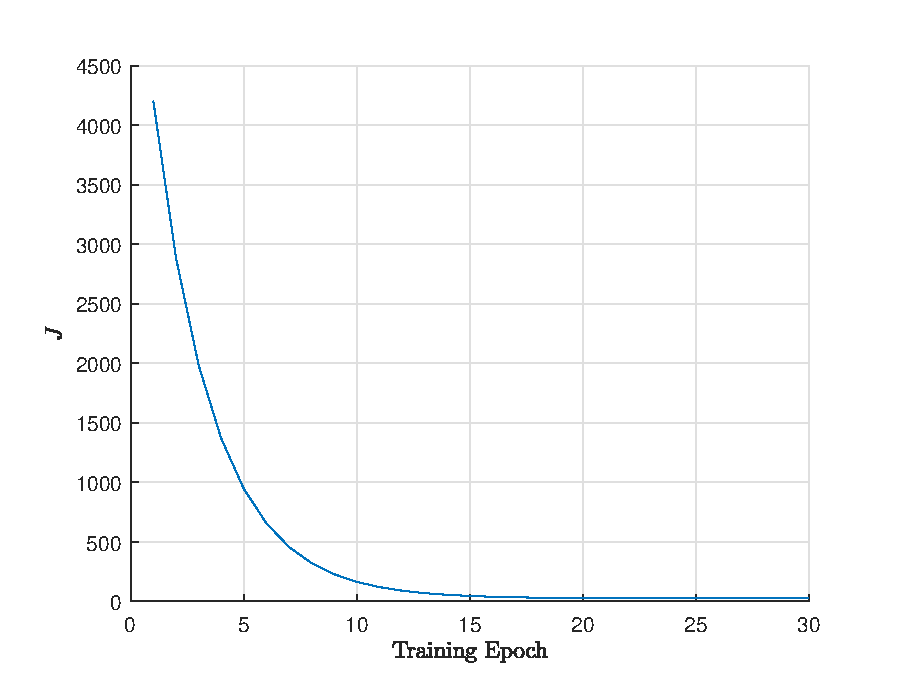
\includegraphics[width=0.6\textwidth]{chapters/part-1/figures/linear_regression_exp_j.eps}
	\caption{The decrement of the cost function during training.} \label{fig:linear_regression_exp_j}
\end{figure}

It is worth mentioning that the quadratic cost function $J$ given by \eqref{eq:linear_regression_solution_j} is a convex function of $\theta$ and $\theta_0$, and there is no local minimum. With a small learning rate $\alpha$, global minimum of $J$ can be achieved.

\subsection{Locally Weighted Regression}

Linear regression handles nonlinear samples by augmenting the feature vector. For example, assume that in \eqref{eq:linear_regression_problem} $f(x, \epsilon)$ is a nonlinear function of $x$, but a linear function of $x_i^2$ where $x_i$ is an element of $x$. In that case $x_i^2$ can be augmented into the features as follows.
\begin{eqnarray}
	\bar{x} &=& \left[x^T, x_i^2\right]^T \nonumber
\end{eqnarray}
and $f(\bar{x}, \epsilon)$ becomes linear to $\bar{x}$. In practice, it can be challenging sometimes to find the most appropriate set of features.

There are other methods to handle nonlinear samples mapping that are very close to linear regression. As an example, \mync{locally weighted regression} segments the samples into piece-wise neighborhoods, applies weighted linear regression for each neighborhood, and then aggregate the results. In each weighted regression corresponding with a neighborhood, each sample is assigned with a weight $0<w^i<1$ when performing weighted least squares in the linear regression. The closer a sample to the center of the neighborhood, the higher the weight. The weight is often calculated by
\begin{eqnarray}
	w_c^{(i)} &=& e^{-\frac{1}{2}(x^{(i)}-x_c)^T\Sigma_c^{-1}(x^{(i)}-x_c)} \nonumber
\end{eqnarray}
where $x_c$ is the center of a neighborhood, and $w_c^{(i)}$ the weight of a sample corresponding with that neighborhood. Scale parameter $\Sigma_c$ depends on the size of the neighborhood.

Locally weighted regression is effective when in the samples are piece-wise linear. Apparently, choosing the number of neighborhoods and their corresponding centers is critical to the algorithm.

Linear regression introduced in Section \ref{sec:linear_regression} is an example of \mync{parametric learning algorithm}, which has a fixed set of parameters $\theta$, $\theta_0$ in \eqref{eq:linear_regression} and the purpose of the machine learning is to fit them with most suitable values. In parametric learning algorithm, since the number of parameters is fixed regardless of the size of the training set, the memory consumption to trace and update the parameters is more or less limited.

Locally weighted regression, on the other hand, is a \mync{non-parametric learning algorithm}. The amount of parameters varies depending on the piece-wise segmentation which is decided by the number and position of the samples. The more and wider spread of sample, the more likely larger number of segments and parameters. 

\section{Logistic Regression}

Logistic regression, though has ``regression'' in its name, is genuinely considered as a binary classification method. 

\subsection{Problem Statement}

Let
\begin{eqnarray}
	y &=& f(x, \epsilon) \nonumber
\end{eqnarray}
where $y \in \{0,1\}$ is the label, $x\in\mathbb{R}^n$ the features, $n$ the number of features, $\epsilon$ the stochasticity of the model, and $f(\cdot)$ an unknown function of $x$. Notice that the label categories the samples into two categories, $0$ (negative) and $1$ (positive).

Linear regression \eqref{eq:linear_regression} cannot fit the labels efficiently. Consider using a non-linear mapping of the following format
\begin{eqnarray}
	h(x) &=& g\left(\theta^Tx\right) \label{eq:logistic_regression}\\
	&=& \dfrac{1}{1+e^{-\theta^Tx}} \nonumber
\end{eqnarray}
where
\begin{eqnarray}
	g(z) &=& \dfrac{1}{1+e^{-z}} \nonumber
\end{eqnarray}
is known as the \mync{sigmoid function} or \mync{logistic function} as shown in Fix \ref{fig:logistic_function}, and $\theta$ is the parameter vector to be fitted. 

\begin{figure}[!htb]
	\centering
	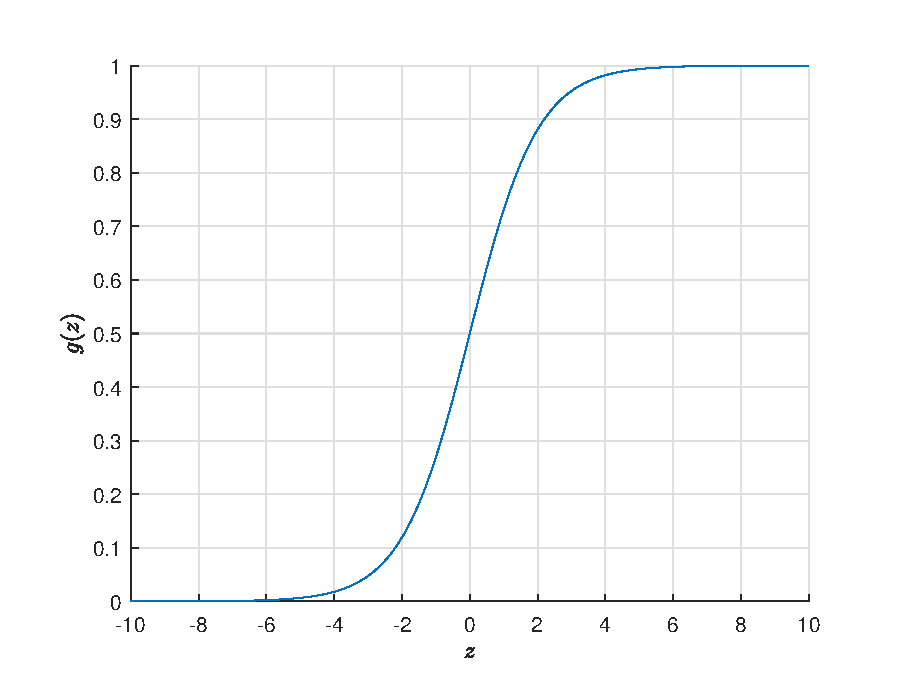
\includegraphics[width=0.6\textwidth]{chapters/part-1/figures/logistic_function.eps}
	\caption{Sigmoid function.} \label{fig:logistic_function}
\end{figure}

The hypothesis $0 < h(x) < 1$ due to the use of the sigmoid function, and it is used to map to the probability of $x$ being categorized with label $y=1$, i.e.,
\begin{eqnarray}
	P(y|x) &\approx& h(x)^y(1-h(x))^{1-y}, y\in\{0,1\} \label{eq:logistic_regression_probability}
\end{eqnarray}

If that can be done, the prediction of the category a new sample $x$ can then be determined by
\begin{eqnarray}
	\hat{y} &=& \left\{\begin{array}{cc}
		0 & h(x) \leq 0.5 \\
		1 & h(x) > 0.5
	\end{array}\right. \nonumber
\end{eqnarray}

\subsection{Solution with Gradient Descent}

As a first step, collect training samples. Let there be $m$ training samples denoted by $(x^{(i)}, y^{(i)})$, $i=1,\ldots,m$. Notice that $y^{(i)} \in \{0,1\}$, some of which taking positive values and others negative values.

Consider using maximum likelihood estimation to determine $\theta$. From \eqref{eq:logistic_regression} and \eqref{eq:logistic_regression_probability}, the likelihood of $\theta$ is given by
\begin{eqnarray}
	\mathcal{L}(\theta) &=& \prod_{i=1}^{m} \left[ h\left(x^{(i)}\right)^{y^{(i)}}\left(1-h\left(x^{(i)}\right)\right)^{1-y^{(i)}}\right] \label{eq:logistic_regression_mle1}
\end{eqnarray}
Maximizing \eqref{eq:logistic_regression_mle1} is equivalent with minimizing
\begin{eqnarray}
	J &=& - \mathrm{log}\left(\mathcal{L}(\theta)\right) \nonumber \\
	&=& - \sum_{i=1}^{m} \left[y^{(i)}h\left(x^{(i)}\right) + \left(1-y^{(i)}\right)\left(1-h\left(x^{(i)}\right)\right)\right] \label{eq:logistic_regression_mle2}
\end{eqnarray}

Consider using batch gradient descent to minimize \eqref{eq:logistic_regression_mle2} as follows
\begin{eqnarray}
	\theta &\leftarrow& \theta - \alpha \dfrac{\partial}{\partial \theta}J \nonumber
\end{eqnarray}
with $\alpha$ the learning rate and from \eqref{eq:logistic_regression_mle2}
\begin{eqnarray}
	\dfrac{\partial}{\partial \theta}L(\theta) &=& \sum_{i=1}^m \left[\left(h\left(x^{(i)}-y^{(i)}\right)\right)x^{(i)}\right] \label{eq:logistic_regression_gradient}
\end{eqnarray}

Notice that similar with the case of linear regression, \eqref{eq:logistic_regression_mle2} has no local maximum other than the global maximum.

One may notice that \eqref{eq:linear_regression_gradient} and \eqref{eq:logistic_regression_gradient} look similar regardless of how $h(x)$ is defined. This is not a coincidence. Though being two different algorithms, they both belong to a super-set algorithm. 

